\section{Casi d'uso}

\subsection{Obiettivi}
La sezione 3 Casi d'uso ha come obiettivo l'identificazione e la descrizione di tutti i casi d'uso, ovvero interazioni tra sistema ed attori, individuati dagli analisti nel tempo tramite lo studio del capitolato d'appalto, del dominio, e tramite incontri con il committente.

\subsection{Attori}
Dato che il requisito obbligatorio richiede la costruzione di una pagina di login che presenti un sistema in grado di distinguere un utente umano da un robot, il prodotto presenterà due tipologie principali di attori:
\begin{center}
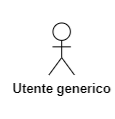
\includegraphics[scale = 1]{img/utente_generico.png}\\
\end{center}
L'utente generico, che potrà essere una persona fisica o anche un bot, potrà accedere a tutte le funzionalità della WebApp. \\
\begin{center}
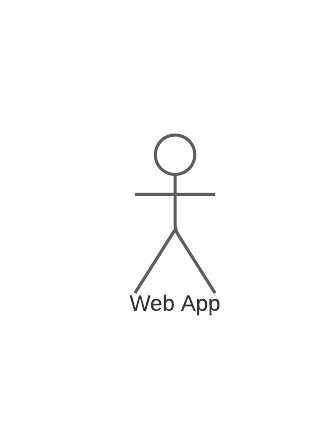
\includegraphics[scale = 1]{img/webapp.png}\\
\end{center}
La WebApp, che potrà accedere alle funzionalità offerte dal servizio CAPTCHA. \\

\subsection{WebApp}

\begin{figure}[H]
    \centering
    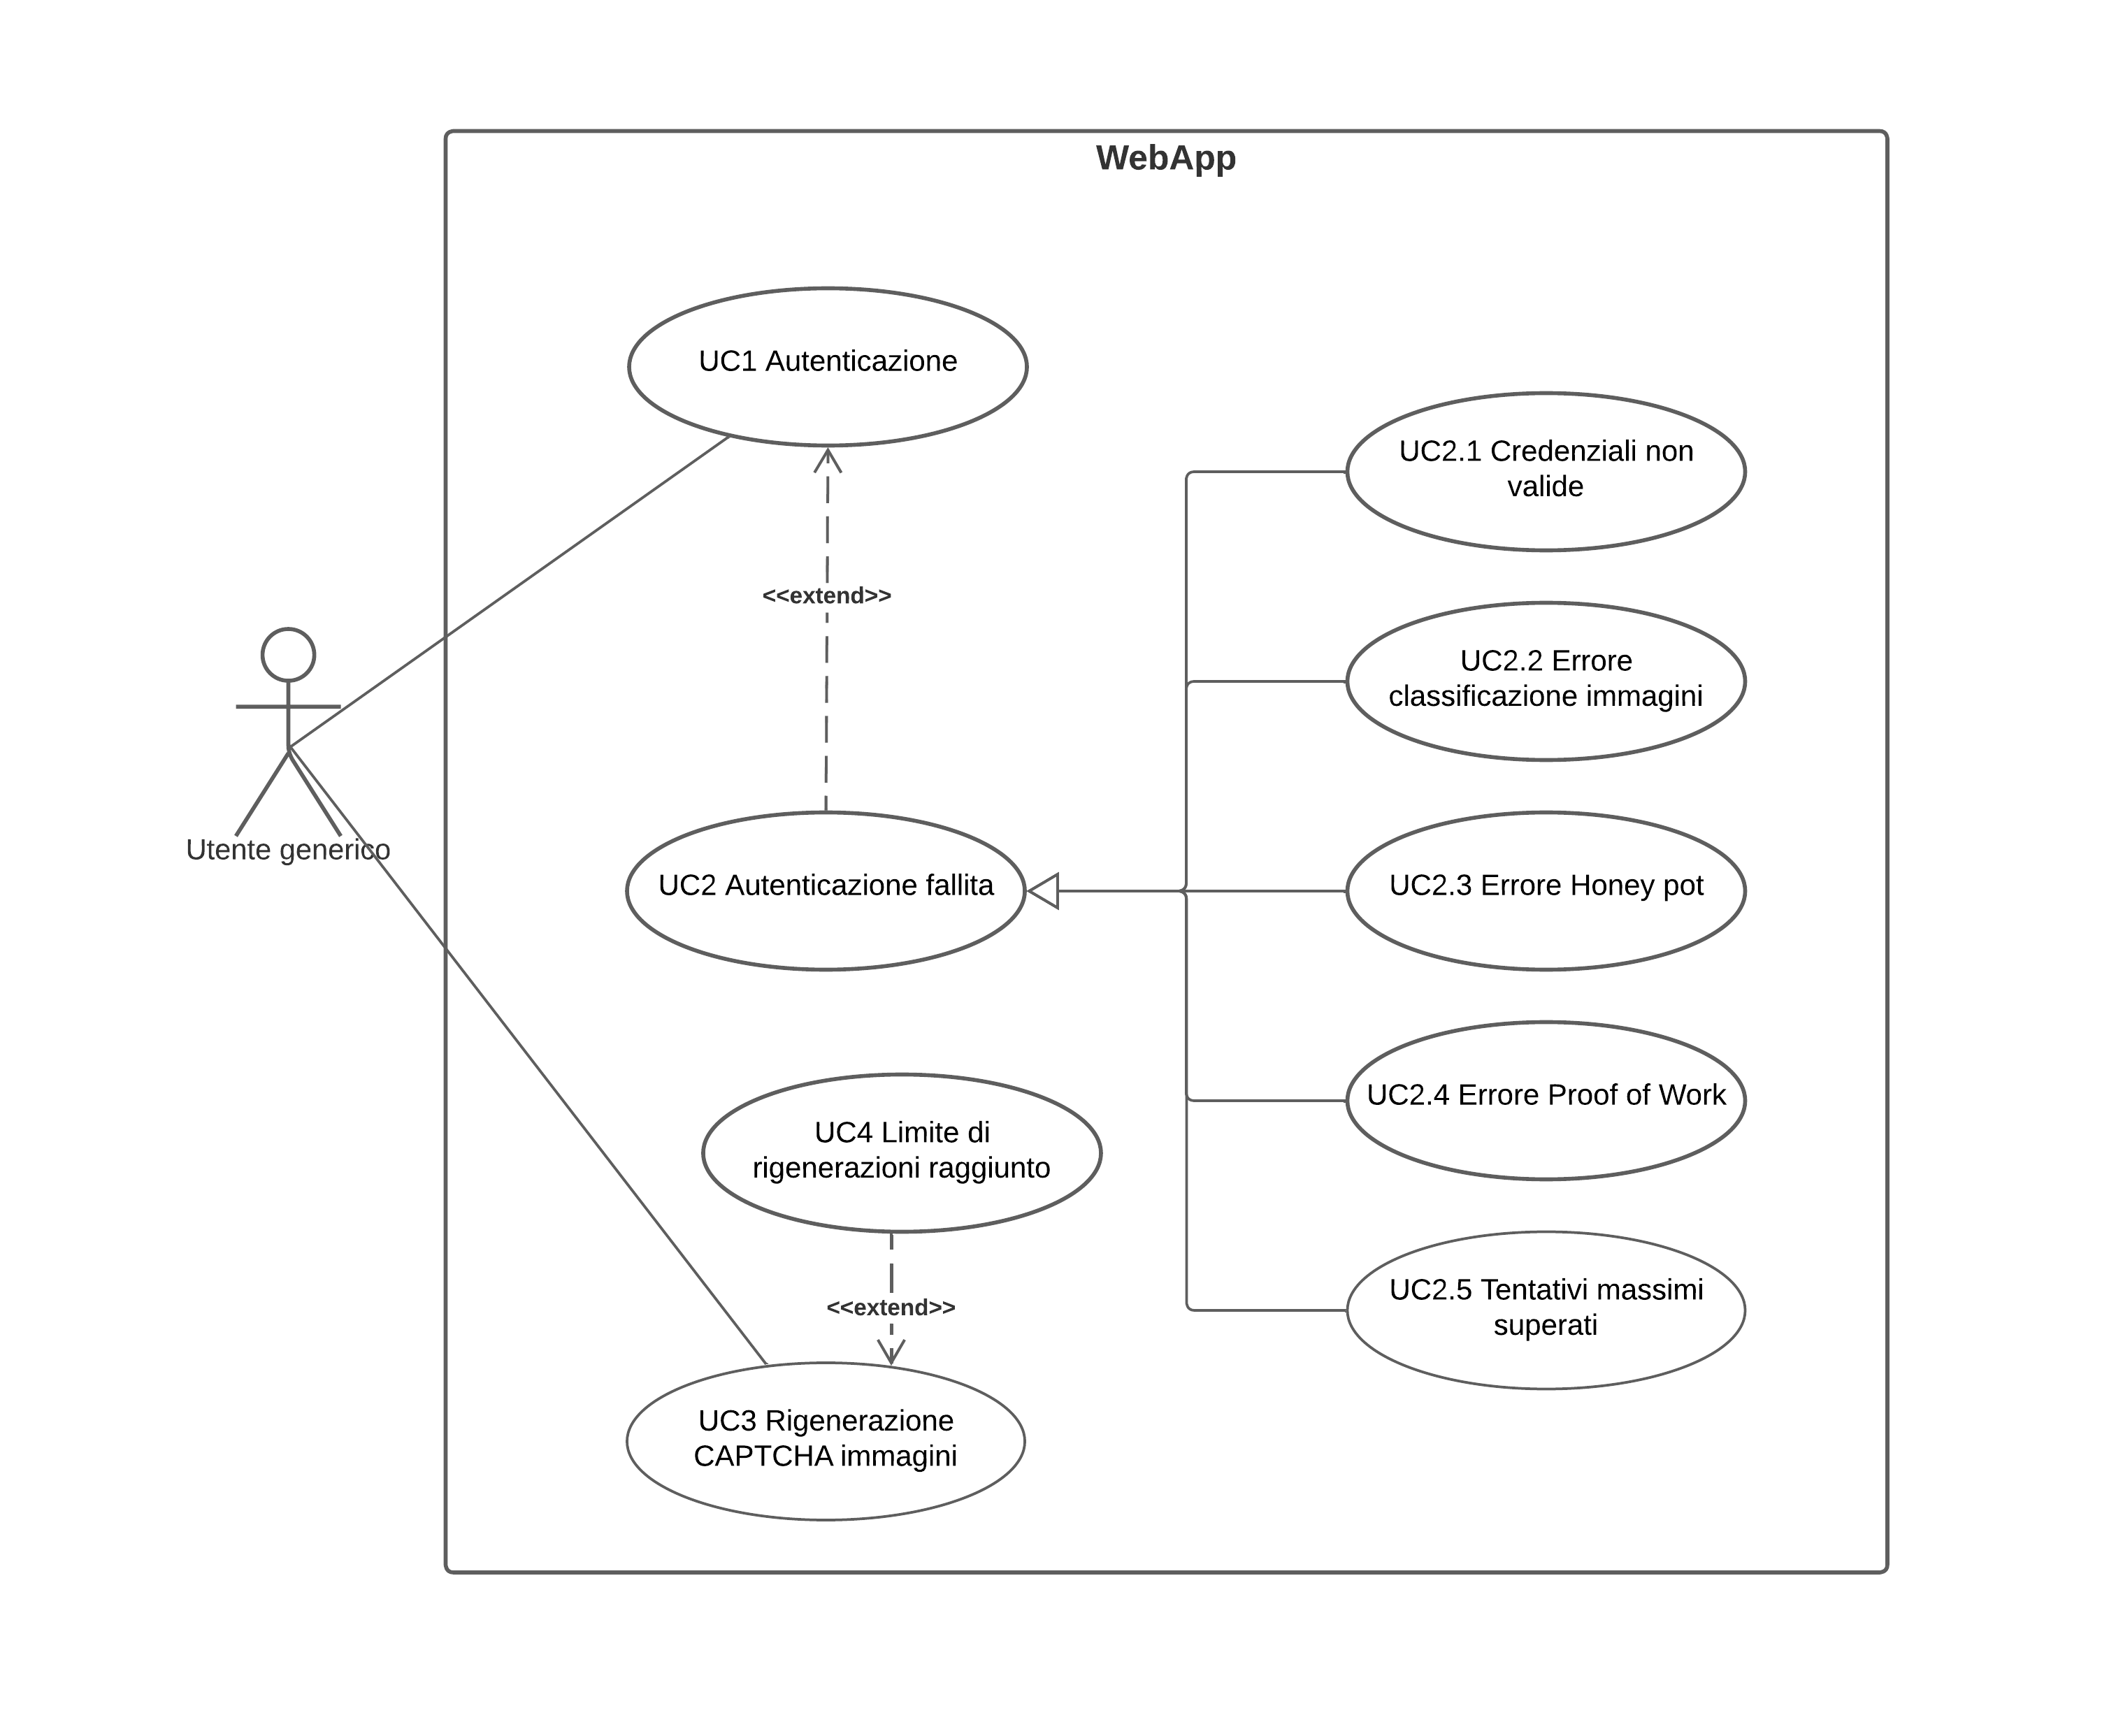
\includegraphics[scale=0.4]{img/web_app.png}
    \caption{Webapp}
\end{figure}

\subsubsection{UC1 - Autenticazione}
\textbf{Attore primario}: Utente generico.\\
\textbf{Precondizioni}: Il sistema non riconosce l'utente.\\
\textbf{Postcondizioni}: L'utente è autenticato nel sistema.\\

\textbf{Scenario principale}: L'utente:
\begin{enumerate}
\item Inserisce le credenziali d'accesso [UC1.1];
\item Compila il CAPTCHA immagini [UC1.2];
\item Supera l'honeypot [UC1.3];
\item Calcola il proof of work [UC1.4].
\end{enumerate}

\textbf{Scenari alternativi}:
\begin{enumerate}
    \item L’utente non supera l'autenticazione [UC2].
\end{enumerate}

\begin{figure}[H]
    \centering
    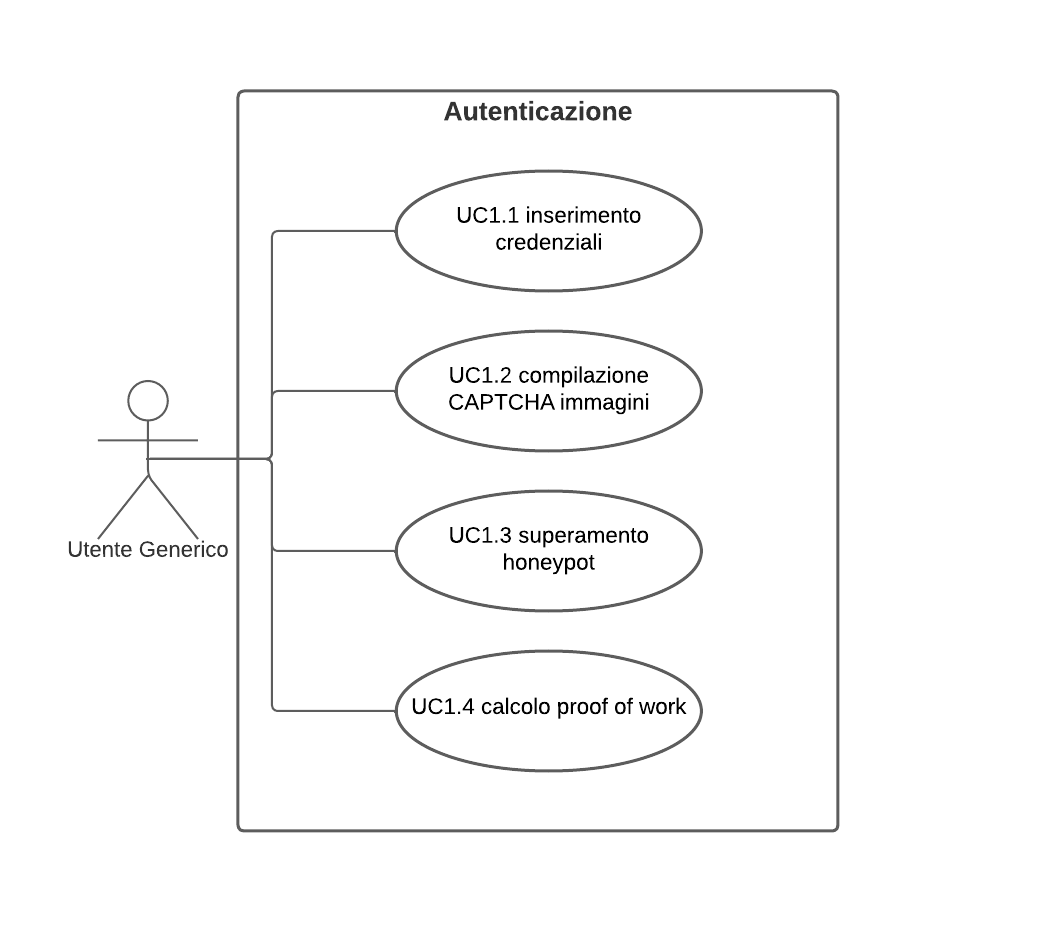
\includegraphics[scale=0.8]{img/Autenticazione.png}
    \caption{UC1-Autenticazione}
\end{figure}

\paragraph{UC1.1 - Inserimento credenziali}
\textbf{Attore primario}: Utente generico.\\
\textbf{Precondizioni}: Il sistema non riconosce l'utente.\\
\textbf{Postcondizioni}: Il sistema ha ricevuto le credenziali dell'utente.\\

\textbf{Scenario principale}: L'utente:
\begin{enumerate}
   \item Inserisce il proprio username;
   \item Inserisce la propria password.
\end{enumerate}

\paragraph{UC1.2 - Compilazione CAPTCHA immagini}
\textbf{Attore primario}: Utente generico.\\
\textbf{Precondizioni}: L'utente visualizza il CAPTCHA immagini proposto dal sistema.\\
\textbf{Postcondizioni}: L'utente ha risolto il CAPTCHA immagini, non necessariamente in modo corretto.\\

\textbf{Scenario principale}: L'utente:
\begin{enumerate}
   \item Visualizza le immagini distorte appartenenti al CAPTCHA;
   \item Classifica le immagini visualizzate secondo il proprio giudizio, che può non corrispondere totalmente alla classificazione in uso dal sistema.
\end{enumerate}

\paragraph{UC1.3 - Superamento honeypot}
\textbf{Attore primario}: Utente generico.\\
\textbf{Precondizioni}: All'utente viene presentata una trappola honeypot.\\
\textbf{Postcondizioni}: L'utente supera l'honeypot.\\

\textbf{Scenario principale}:
\begin{enumerate}
   \item All'utente viene presentata una trappola honeypot, sottoforma di immagine nascosta ad un utente umano, ma visibile ad un bot.
   \item L'utente non seleziona l'immagine nascosta.
\end{enumerate}

\paragraph{UC1.4 - Calcolo proof of work}
\textbf{Attore primario}: Utente generico.\\
\textbf{Precondizioni}: All'utente viene richiesto il calcolo del proof of work.\\
\textbf{Postcondizioni}: Il proof of work viene calcolato.\\

\textbf{Scenario principale}:
\begin{enumerate}
   \item Viene calcolato il proof of work;
   \item Il risultato viene fornito al sistema.
\end{enumerate}

\subsubsection{UC2 - Autenticazione fallita}
\textbf{Attore primario}: Utente generico.\\
\textbf{Precondizioni}: L’utente ha commesso un errore durante l'autenticazione.\\
\textbf{Postcondizioni}:L’utente visualizza un messaggio di errore e l’operazione di autenticazione fallisce.\\

\textbf{Scenario principale}:
\begin{enumerate}
   \item L’utente commette un errore nella compilazione del modulo di login;
   \item L'utente visualizza un messaggio di errore;
   \item L'utente non viene autenticato nel sistema.
\end{enumerate}

\textbf{Generalizzazioni}: L'utente ha commesso uno dei seguenti errori:
\begin{enumerate}
	\item Ha inserito delle credenziali errate [UC2.1]
	\item Ha sbagliato la classificazione delle immagini [UC2.2]
	\item E' caduto nella trappola honeypot [UC2.3]
	\item Non ha calcolato il proof of work [UC2.4]
	\item Ha superato il numero massimo di tentativi disponibili [UC2.5]
\end{enumerate}

\paragraph{UC2.1 - Credenziali errate}
\textbf{Attore primario:} Utente generico.\\
\textbf{Precondizioni}: L’utente non ha inserito le credenziali corrette.\\
\textbf{Postcondizioni}: L’utente visualizza un messaggio di errore e l’operazione di autenticazione fallisce.\\

\textbf{Scenario principale}:
\begin{enumerate}
    \item L'utente inserisce uno username non registrato nel sistema, una password sbagliata per lo username scelto, oppure non inserisce le credenziali;
	\item L’utente visualizza un messaggio di errore;
	\item Il numero di tentativi consecutivi compiuti dall’utente aumenta di 1.
\end{enumerate}

\paragraph{UC2.2 - Errore classificazione immagini}
\textbf{Attore primario:} Utente generico.\\
    \textbf{Precondizioni}: L’utente non ha compilato correttamente il CAPTCHA immagini.\\
\textbf{Postcondizioni}: L’utente visualizza un messaggio di errore e l’operazione di autenticazione fallisce.\\

\textbf{Scenario principale}:
\begin{enumerate}
    \item L'utente classifica le immagini proposte superando il margine di errore consentito rispetto alla classificazione in uso dal sistema;
	\item L’utente visualizza un messaggio di errore;
	\item Il numero di tentativi consecutivi compiuti dall’utente aumenta di 1.
\end{enumerate}

\paragraph{UC2.3 - Errore honeypot}
\textbf{Attore primario:} Utente generico.\\
\textbf{Precondizioni}: L’utente ha selezionato l'immagine nascosta.\\
\textbf{Postcondizioni}: L’utente visualizza un messaggio di errore e l’operazione di autenticazione fallisce.\\

\textbf{Scenario principale}:
\begin{enumerate}
    \item L'utente seleziona l'immagine nascosta;
	\item L’utente visualizza un messaggio di errore;
	\item L'utente viene riconosciuto come bot e verrà bloccato nei futuri tentativi di login.
\end{enumerate}

\paragraph{UC2.4 - Errore proof of work}
\textbf{Attore primario:} Utente generico\\
\textbf{Precondizioni}: Il proof of work non viene calcolato.\\
\textbf{Postcondizioni}:  L’utente visualizza un messaggio di errore e l’operazione di autenticazione fallisce.\\

\textbf{Scenario principale}:
\begin{enumerate}
    \item L'utente inserisce le credenziali e compila il CAPTCHA immagini in maniera troppo rapida, per cui non viene eseguito il calcolo del proof of work;
	\item L’utente visualizza un messaggio di errore;
	\item L'utente viene riconosciuto come bot e verrà bloccato nei futuri tentativi di login.
\end{enumerate}

\paragraph{UC2.5 - Tentativi massimi superati}
\textbf{Attore primario:} Utente generico.\\
\textbf{Precondizioni}: L'utente ha superato il numero massimo di tentativi consentiti per il login.\\
\textbf{Postcondizioni}: L’utente visualizza un messaggio di errore e l’operazione di autenticazione fallisce.\\

\textbf{Scenario principale}:
\begin{enumerate}
    \item L'utente effettua più tentativi di login consecutivi rispetto a quelli consentiti dal sistema;
	\item L’utente visualizza un messaggio di errore;
	\item L'utente potrà  riprovare ad autenticarsi più tardi.
\end{enumerate}

\subsubsection{UC3 - Rigenerazione CAPTCHA immagini}
\textbf{Attore primario}: Utente generico.\\
\textbf{Precondizioni}: L'utente non riconosce le immagini contenute nel CAPTCHA e pertanto non può procedere con la loro classificazione.\\
\textbf{Postcondizioni}: All'utente viene proposto un nuovo set di immagini da classificare.\\

\textbf{Scenario principale}:
\begin{enumerate}
   \item L'utente non è in grado di classificare le immagini proposte dal sistema;
   \item L'utente richiede un altro set di immagini;
   \item Il sistema genera un nuovo set di immagini e le propone all'utente;
   \item Il numero di rigenerazioni CAPTCHA immagini richieste dall’utente aumenta di 1;
   \item L'utente può procedere con la risoluzione del CAPTCHA immagini.
\end{enumerate}

\subsubsection{UC4 - Limite di rigenerazioni aggiunto}
\textbf{Attore primario:} Utente generico.\\
\textbf{Precondizioni}: L'utente ha superato il numero massimo di richieste di rigenerazione CAPTCHA immagini consentito.\\
\textbf{Postcondizioni}: L’utente visualizza un messaggio di errore e il CAPTCHA immagini non viene rigenerato.\\

\textbf{Scenario principale}:
\begin{enumerate}
    \item L'utente effettua più richieste consecutive di rigenerazione CAPTCHA immagini rispetto a quelle consentite dal sistema;
	\item L’utente visualizza un messaggio di errore.
\end{enumerate}

\subsection{CAPTCHA}

\begin{figure}[H]
    \centering
    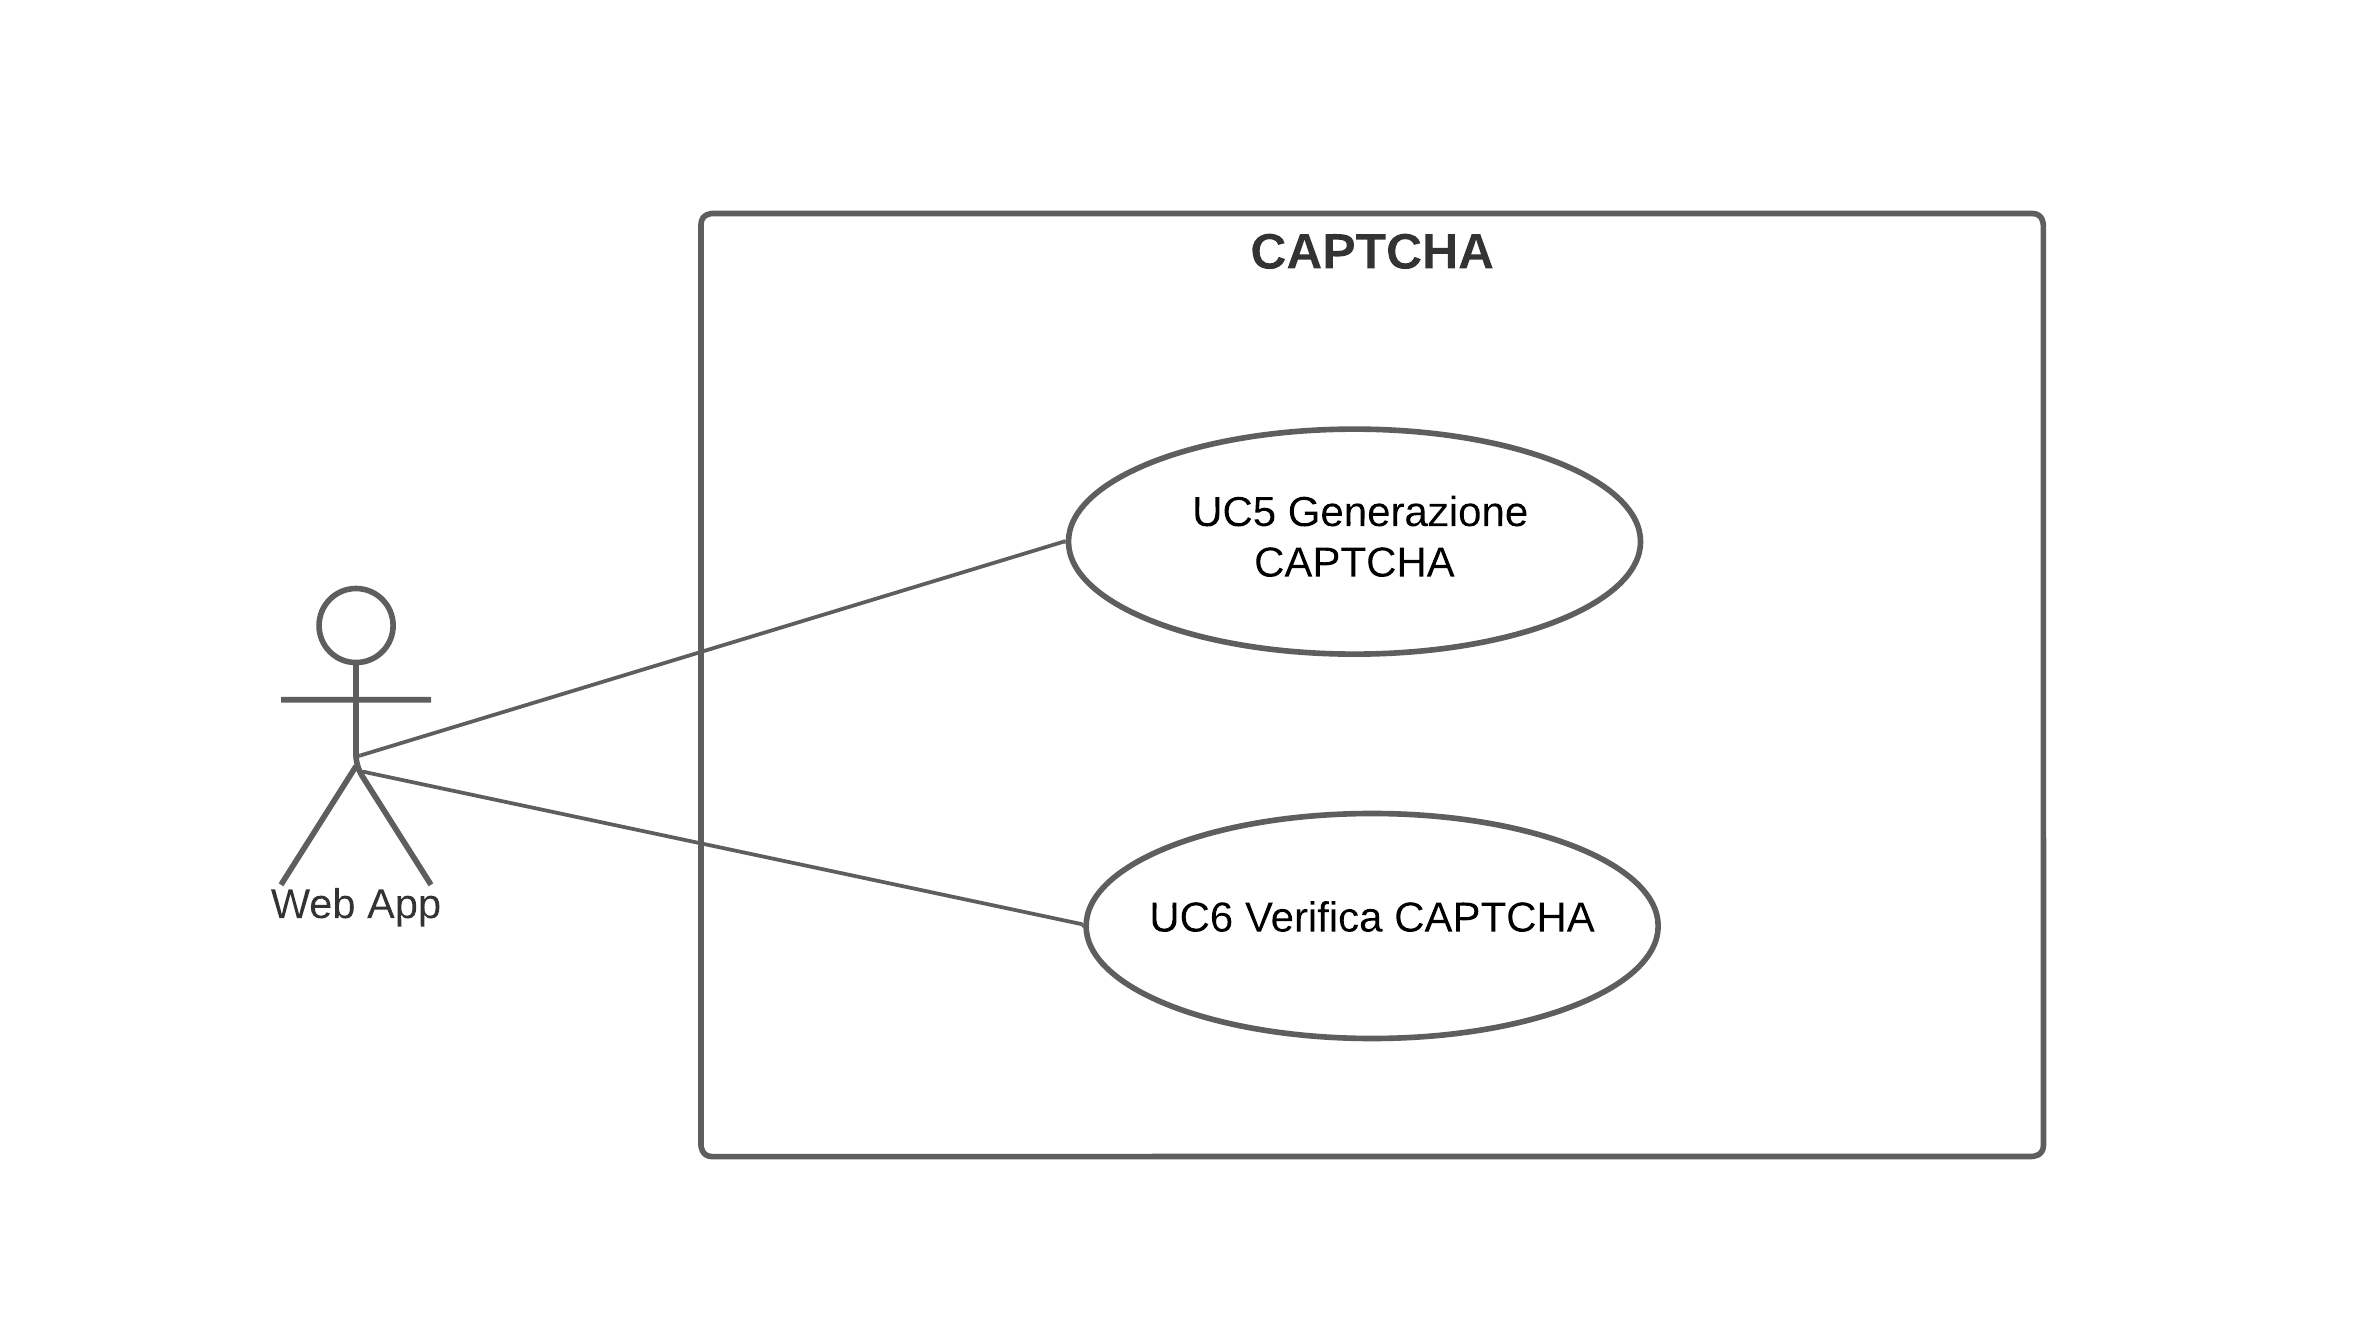
\includegraphics[scale=0.4]{img/captcha.png}
    \caption{Captcha}
\end{figure}


\subsubsection{UC5 - Generazione CAPTCHA immagini}
\textbf{Attore primario:} WebApp.\\
\textbf{Precondizioni}: La WebApp richiede la generazione di un CAPTCHA immagini.\\
\textbf{Postcondizioni}: Il CAPTCHA immagini viene generato e restituito alla WebApp.\\

\textbf{Scenario principale}:
\begin{enumerate}
    \item La WebApp richiede la generazione di un CAPTCHA immagini;
    \item Il CAPTCHA immagini viene generato utilizzando le immagini fornite da Unsplash e quelle presenti nel database interno;
    \item Viene generato un immagine aggiuntivo che funge da honeypot;
    \item Il CAPTCHA immagini viene restituito alla WebApp.
\end{enumerate}
\textbf{Scenari alternativi}:
\begin{enumerate}
    \item Il CAPTCHA non può essere generato [UC6].
\end{enumerate}

\subsubsection{UC6 - Errore generazione CAPTCHA immagini}
\textbf{Attore primario:} WebApp.\\
\textbf{Precondizioni}: La WebApp richiede la generazione di un CAPTCHA immagini.\\
\textbf{Postcondizioni}: Il CAPTCHA immagini non viene generato.\\

\textbf{Scenario principale}:
\begin{enumerate}
    \item La WebApp richiede la generazione di un CAPTCHA immagini;
    \item Errore durante la generazione per motivi:
		\begin{itemize}
    		\item Connessione rete:
			\begin{itemize}
	    		\item Assenza connessione alla rete;
	    		\item Unsplash non risponde alla richiesta;
			\item Interruzione di connessione durante la richiesta.
			\end{itemize}
    		\item Dati scorretti:
			\begin{itemize}
	    		\item Immagine richiesta non presente;
	    		\item Immagine richiesta ha un formato non supportato.
			\end{itemize}
		\end{itemize}
    \item Il CAPTCHA non viene generato e restituisce un messaggio di errore alla WebApp.\\
\end{enumerate}

\subsubsection{UC7  - Generazione proof of work}
\textbf{Attore primario:} WebApp.\\
\textbf{Precondizioni}: La WebApp richiede la generazione del proof of work.\\
\textbf{Postcondizioni}: Viene generato il proof of work e restituito alla WebApp.\\

\textbf{Scenario principale}:
\begin{enumerate}
    \item La WebApp richiede la generazione del proof of work;
    \item Viene creato il Proof of work per il CAPTCHA per minare crypto valute;
    \item Il proof of work viene restituito alla WebApp.
\end{enumerate}

\subsubsection{UC8 - Verifica CAPTCHA}
\textbf{Attore primario:} WebApp.\\
\textbf{Precondizioni}: La WebApp richiede la verifica CAPTCHA.\\
\textbf{Postcondizioni}: Viene data una risposta alla WebApp.\\

\textbf{Scenario principale}:
\begin{enumerate}
    \item La WebApp richiede la verifica della corretteza del CAPTCHA compilata;
    \item Viene verificata la corretteza di:
    \begin{itemize}
		\item CAPTCHA immagini;
		\item Honeypot;
		\item Proof of Work.
    \end{itemize}
    \item In base alla percentuale della correttezza, viene emesso il risultato e restituito alla WebApp.
\end{enumerate}
